\subsection{Induzierte Abbildung
\label{buch:subsection:induzierte-abbildung}}
Früher haben wurde eine Abbildung $f_*$ zwischen Kettenkomplexen $C_*$ und
$D_*$ so definiert,
dass sie mit den Randoperatoren verträglich sein muss.
Diese Forderung bewirkt, dass sich auch eine lineare Abbildung
\[
H_k(f) \colon H_k(C) \to H_k(D)
\]
zwischen den Homologiegruppen ergibt, wie wir nun zeigen wollen.

\subsubsection{Definition der induzierten Abbildung}
Um eine Abbildung von $H_k(C)$ nach $H_k(D)$ zu definieren, müssen wir
zu einem Element von $H_k(C)$ ein Bildelement konstruieren.
Ein Element in $H_k(C)$ ist eine Menge von Zyklen in $Z^C_k$, die sich
nur um einen Rand in $B_k$ unterscheiden.
Wir wählen also einen Zyklus $z\in Z_k$ und bilden ihn auf $f_k(z)$ ab.
Wegen $\partial^D_kf(z)=f\partial^C_kz = f(0) =0 $ ist auch $f_k(z)$
ein Zyklus.
Wir müssen jetzt aber noch zeigen, dass eine andere Wahl des Zyklus
das gleiche Element in $H_k(D)$ ergibt.
Dazu genügt es zu sehen, dass sich $f(z)$ höchstens um einen Rand
ändert, wenn man $z$ um einen Rand ändert.
Sei also $b\in B^C_k$ ein Rand, d.~h.~es gibt ein $w\in C_{k+1}$ mit
$\partial^C_{k+1}w=b$.
Dann gilt aber auch
\[
f_k(z+b)
=
f_k(z) + f_k(b)
=
f_k(z) + f_k(\partial^C_{k+1}w)
=
f_k(z) + \partial^D_{k+1}(f_k(w)).
\]
Der letzte Term ist ein Rand in $D_k$, somit ändert sich $f_k(z)$ nur
um diesen Rand, wenn man $z$ um einen Rand ändert.
$f_k(z)$ und $f_k(z+b)$ führen auf die selbe Homologieklasse.

\subsubsection{Matrixdarstellung}
In Abschnitt~\ref{buch:subsection:basiswahl} wurde gezeigt, wie man
für die Vektorräume der Zyklen eine Basis derart finden kann, 
dass die Ränder von einer Teilmenge der Basis aufgespannt werden.
Eine solche Basis kann man immer erweitern zu einer Basis von $C_k$.
Für das Folgende bezeichnen wir die Vektoren einer solche Basis von $C_k$ 
mit
\[
\{
b_1,\dots, b_r,
z_1,\dots,z_l,
c_1,\dots,c_s
\}.
\]
wobei die Vektoren  die folgende Bedeutung haben:
\begin{center}
\begin{tabular}{|l|p{9cm}|}
\hline
Vektoren&Bedeutung\\
\hline
$b_1,\dots,b_r$ & Basis für $B_k(C)$ \\
$z_1,\dots,z_l$ &{\raggedright zusätzliche Vektoren für eine Basis von $Z_k(C)$, Repräsentanten für eine Basis von $H_k(C)$}\\
$c_1,\dots,c_s$ & zusätzliche Vektoren für eine Basis von $C_k$ \\
\hline
\end{tabular}
\end{center}

Wählt man eine Basis dieser Art sowohl in $C_*$ wie auch in $D_*$,
dann kann man die induzierte Abbildung als $3\times 3$-Blockmatrix
schreiben.
Man verwendet dabei, dass $f_k$ die Unterräume $B_k(C)$ und
$Z_k(C)$ in die entsprechenden Unterräume $B_k(D)$ und $Z_k(D)$
abbildet, also
\[
f_k(B_k(C)) \subset B_k(D)
\qquad\text{und}\qquad
f_k(Z_k(C)) \subset Z_k(D).
\]
In der Matrixdarstellung äussert sich das darin, dass die Blöcke
links unten zu Null werden.
Die Matrixdarstellung von $f_k$ hat daher die Form
\[
f_k
=
\begin{pmatrix}
f_{k,B} &    *    & * \\
   0    & f_{k,Z} & * \\
   0    &    0    & f_{k,*}
\end{pmatrix}.
\]
Genauso kann man natürlich auch die Randoperatoren in dieser Basis
ausdrücken.
Sie bilden die Zyklen auf $0$ ab und aus den Vektoren $c_1,\dots,c_s$
werden Ränder.
Die Matrix hat daher die Form
\[
\partial_k
=
\begin{pmatrix}
0& 0 & \Delta_k \\
0& 0 & 0 \\
0& 0 & 0
\end{pmatrix}
\]
\begin{figure}
\centering
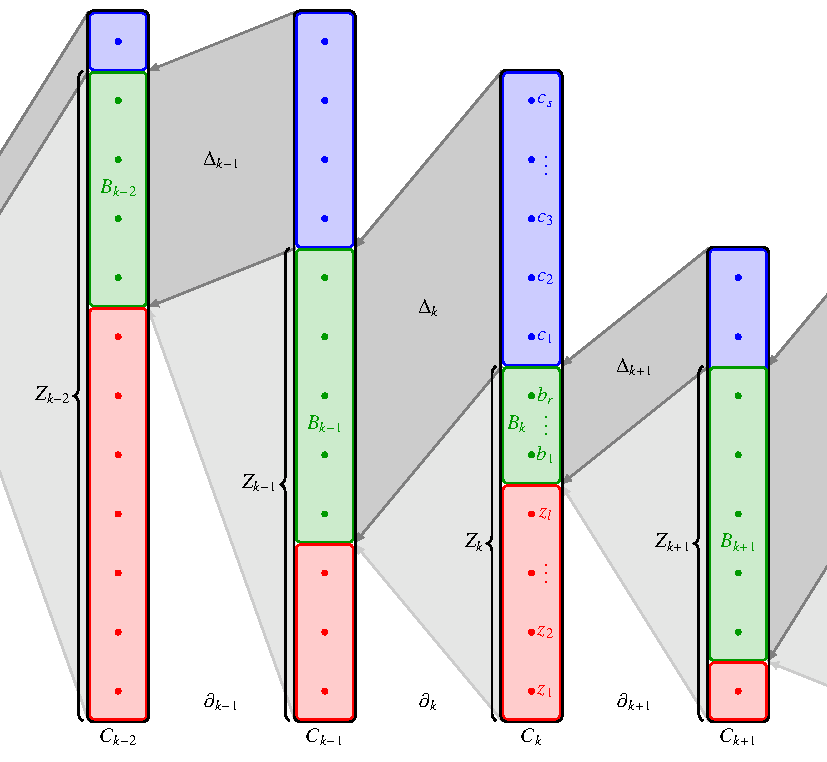
\includegraphics{chapters/95-homologie/images/complexbasis.pdf}
\caption{Basiswahl für den Kettenkomplex $C_k$.
Der Randoperator $\partial_k$ bildet $Z_k$ auf $0$ ab, der blaue
Unterraum, aufgespannt von den Vektoren $c_i$, wird bijektiv auf $B_{k-1}$
abgebildet.
Eine Basis kann immer so gefunden werden, dass die Vektoren $c_i$ 
von $\partial_k$ auf die Basisvektoren von $B_{k-1}$ abgebildet werden.
In dieser Basis ist $\Delta_k$ eine Einheitsmatrix.
\label{buch:homologie:fig:komplexbasis}}
\end{figure}%
Die Bedingung \eqref{buch:komplex:abbildung} in Definition~\ref{buch:komplex:def:abbildung}
für die Abbildung von Kettenkomplexen
bekommt jetzt die Matrixform
\begin{equation}
\left.
\begin{aligned}
\partial_k^{D}\circ f_k
&=
\begin{pmatrix}
0&0&\Delta_k^{(D)}\\
0&0&0\\
0&0&0
\end{pmatrix}
\begin{pmatrix}
f_{k,B} &    *    & * \\
   0    & f_{k,Z} & * \\
   0    &    0    & f_{k,*}
\end{pmatrix}
=
\begin{pmatrix}
0&0&\Delta_k^{(D)}f_{k,*}\\
0&0&0\\
0&0&0
\end{pmatrix}
\\
f_{k-1}\circ \partial_k^C
&=
\begin{pmatrix}
f_{k-1,B}&   *   &   *   \\
   0   &f_{k-1,Z}&   *   \\
   0   &   0   &f_{k-1,*}
\end{pmatrix}
\begin{pmatrix}
0&0&\Delta_k^{(C)}\\
0&0&0\\
0&0&0
\end{pmatrix}
=
\begin{pmatrix}
0&0&f_{k-1,B}\Delta_k^{(C)}\\
0&0&0\\
0&0&0
\end{pmatrix}
\end{aligned}
\right\}
\Rightarrow
\Delta_k^{(D)}f_{k,*}
=
f_{k-1,B}\Delta_k^{(C)}.
\label{buch:homologie:matrixform}
\end{equation}
Für die induzierte Abbildung in Homologie ist ausschliesslich der
Block $f_{k,Z}$ notwendig, die Matrix von $H_k(f)$ in der gewählten
Basis von $H_k(C)$ bzw.~$H_k(D)$ ist also genau die Matrix $f_{k,Z}$.


Wie Abbildung~\ref{buch:homologie:fig:komplexbasis} illustriert, können die
Basisvektoren $c_*$ in $C_k$ so gewählt werden, dass sie vom Randoperator
$\partial_k$ auf die Basisvektoren von $Z_{k-1}$ abgebildet werden.
Bei dieser Wahl wird die Matrix $\Delta_k$ eine Einheitsmatrix.

\subsubsection{Spur}
Wir betrachten jetzt den Fall einer Selbstabbildung $f_*\colon C_*\to C_*$.
Die Basis soll so gewählt werden, dass $\Delta_k$ eine Einheitsmatrix ist.
Aus~\eqref{buch:homologie:matrixform} kann man ablesen, dass für diese
Basiswahl $f_{k,*}=f_{k-1,B}$ gilt.
Die Matrizen von $f_k$ haben daher die Form
\[
f_k
=
\begin{pmatrix}
f_{k,B} &    *    & * \\
   0    & f_{k,Z} & * \\
   0    &   0     & f_{k-1,B}
\end{pmatrix}.
\]
Entsprechend ist die Spur
\begin{equation}
\operatorname{Spur} f_k
=
\operatorname{Spur} f_{k,B}
+
\operatorname{Spur} f_{k,Z}
+
\operatorname{Spur} f_{k-1,B}.
\label{buch:homologie:eqn:spur}
\end{equation}



